\documentclass[10pt, xetex, hyperref={pdfpagelabels=false}]{beamer}

% -------------------------------------------------------------------
% Packages
% -------------------------------------------------------------------
\usepackage[english]{babel}
\usepackage{amsmath, amsthm, amssymb}

\newtheorem{mainth}{Theorem}{\bfseries}{\rmfamily}
% \newtheorem{mainlemma}[mainth]{Lemma}{\bfseries}{\rmfamily}
% \newtheorem{mydefinition}[mainth]{Definition}{\bfseries}{\rmfamily}
% \newtheorem{myexamplenum}[mainth]{Example}{\bfseries}{\rmfamily}

% \newtheorem*{notation}{Notation}{\it}{\rmfamily}
% \newtheorem*{myremark}{Remark}{\bfseries}{\rmfamily}

% -------------------------------------------------------------------
% Natural deduction proofs
% -------------------------------------------------------------------
\usepackage{bussproofs}
\EnableBpAbbreviations
\def\extraVskip{3pt}

% https://tex.stackexchange.com/questions/104554/
% how-to-scale-prooftree-environment-bussproofs-package
\newenvironment{scprooftree}[1]%
  {\gdef\scalefactor{#1}\begin{center}\proofSkipAmount \leavevmode}%
  {\scalebox{\scalefactor}{\DisplayProof}\proofSkipAmount \end{center}}

% -------------------------------------------------------------------
% -- Algorithms
% -------------------------------------------------------------------
\usepackage{algorithm,algpseudocode}

% -------------------------------------------------------------------
% \usepackage{fancyvrb}
\usepackage{geometry}
\usepackage{graphicx}
\usepackage{lmodern}
\usepackage{url}

% --------------------------------------------------------------------
% Color definitions.
% --------------------------------------------------------------------
\usepackage{xcolor}
\definecolor{aliceblue}{rgb}{0.94, 0.97, 1.0}
\definecolor{amber}{rgb}{1.0, 0.75, 0.0}
\definecolor{amethyst}{rgb}{0.6, 0.4, 0.8}
\definecolor{antiquefuchsia}{rgb}{0.57, 0.36, 0.51}
\definecolor{ashgrey}{rgb}{0.7, 0.75, 0.71}
\definecolor{background}{RGB}{1,0,102}
\definecolor{ballblue}{rgb}{0.13, 0.67, 0.8}
\definecolor{bline}{RGB}{255, 255, 255}
\definecolor{blue(munsell)}{rgb}{0.0, 0.5, 0.69}
\definecolor{blue(pigment)}{rgb}{0.2, 0.2, 0.6}
\definecolor{blu}{RGB}{1,0,102}
\definecolor{bondiblue}{rgb}{0.0, 0.58, 0.71}
\definecolor{brightmaroon}{rgb}{0.76, 0.13, 0.28}
\definecolor{cadet}{rgb}{0.33, 0.41, 0.47}
\definecolor{darkgreen}{rgb}{0.0, 0.5, 0.0}
\definecolor{darkred}{rgb}{0.5, 0.0, 0.13}
\definecolor{decoration}{RGB}{10,164,216}
\definecolor{fontc}{RGB}{255, 255, 255}
\definecolor{logo}{RGB}{1,0,102}

% --------------------------------------------------------------------
% My palette.
% --------------------------------------------------------------------
\definecolor{energy}{RGB}{49,247,250}
\definecolor{delicate}{RGB}{67,179,223}
\definecolor{faded}{RGB}{76,117,195}
\definecolor{plum}{RGB}{87,78,164}
\definecolor{petunias}{RGB}{109,80,139}
\definecolor{letour}{RGB}{101,41,105}

% --------------------------------------------------------------------
% Beamer configuration.
% --------------------------------------------------------------------
\usetheme{default}
\usecolortheme{default}

\beamertemplatenavigationsymbolsempty
\setbeamertemplate{navigation symbols}{}
\hypersetup{pdfpagemode=UseNone}

% footer.
\setbeamercolor{headFoot}{fg=gray, bg=white}

\setbeamertemplate{footline}{
  \leavevmode%
  \hbox{%
  % \begin{beamercolorbox}
  %   [wd=.8\paperwidth,ht=2.3ex,dp=1ex,left]{headFoot}%
  %   \hspace*{2ex}\textbf\insertshorttitle\hspace*{2mm}|
  %   \hspace*{2mm}\textbf\insertshortauthor
  % \end{beamercolorbox}%
  \begin{beamercolorbox}
    [wd=\paperwidth,ht=2.4ex,dp=1ex,right]{headFoot}%
    \insertframenumber{}/\inserttotalframenumber\hspace*{2ex}
  \end{beamercolorbox}}%
  \vskip 0pt%
}

\setbeamerfont{frametitle}{series=\bfseries}
\setbeamercolor{frametitle}{fg=white,bg=blu}

\setbeamerfont{framesubtitle}{size=\normalfont\scriptsize}
\setbeamercolor{framesubtitle}{fg=white, bg=blu}

\setbeamercolor{background canvas}{bg=white}
\setbeamercolor{normal text}{fg=black}

% \setbeamercolor{institute}{fg=blu}
\setbeamercolor{title}{fg=blu}
% \setbeamercolor{subtitle}{fg=blu}

% \setbeamercolor{titlelike}{fg=blu}
\setbeamerfont{footnote}{size=\tiny}
\setbeamercolor{footnote}{fg=gray}
% \setbeamercolor{block title}{bg=blu,fg=blu}
% \setbeamercolor{block body}{bg=aliceblue}
\setbeamercolor{item}{fg=blu} % color of bullets
\setbeamercolor{subitem}{fg=blu}
% \setbeamercolor{itemize/enumerate subbody}{fg=blu}
% \setbeamertemplate{itemize subitem}{{\textendash}}
% \setbeamerfont{itemize/enumerate subbody}{size=\footnotesize}
% \setbeamerfont{itemize/enumerate subitem}{size=\footnotesize}

% --------------------------------------------------------------------
% Fonts
% --------------------------------------------------------------------
\usefonttheme{professionalfonts}
% \usefonttheme{serif}

\usepackage{fontspec}
\usepackage{mathtools}
\usepackage{unicode-math}

\newfontfamily\djvu[ExternalLocation=fonts/
  , BoldFont=DejaVuSansMono-Bold.ttf
  , BoldItalicFont=DejaVuSansMono-BoldOblique.ttf
  , ItalicFont=DejaVuSansMono-Oblique.ttf
  ]{DejaVuSansMono.ttf}


\newfontfamily\djvumathfont[ExternalLocation=fonts/,
, BoldFont=DejaVuSansMono-Bold.ttf
, BoldItalicFont=DejaVuSansMono-BoldOblique.ttf
, ItalicFont=DejaVuSansMono-Oblique.ttf
]{DejaVuMathTeXGyre.ttf}

% \setmonofont[ExternalLocation=fonts/
% , BoldFont=DejaVuSansMono-Bold.ttf
% , BoldItalicFont=DejaVuSansMono-BoldOblique.ttf
% , ItalicFont=DejaVuSansMono-Oblique.ttf
% ]{DejaVuSansMono.ttf}

% \setmathfont[ExternalLocation=fonts/
%   ]{DejaVuMathTeXGyre.ttf}
% \newfontfamily\mathfont{fonts/DejaVuMathTeXGyre.ttf}

% \setmainfont[ExternalLocation=fonts/
%   , BoldFont=SourceSansPro-Semibold.otf
%   , BoldItalicFont=SourceSansPro-SemiboldIt.otf
%   , ItalicFont=SourceSansPro-It.otf
%   ]{SourceSansPro-Regular.otf}

\newfontfamily\sourcecode[ExternalLocation=fonts/
  , BoldFont=SourceCodePro-Semibold.ttf
  , BoldItalicFont=SourceCodePro-SemiboldIt.ttf
  , ItalicFont=SourceCodePro-It.ttf
  ]{SourceCodePro-Regular.ttf}

%following lines borrowed from cmbright.sty
% \DeclareSymbolFont      {operators} {OT1}{cmbr}{m}{n}
% \DeclareSymbolFont        {letters} {OML}{cmbrm}{m}{it}
% \SetSymbolFont      {letters}{bold} {OML}{cmbrm}{b}{it}
% \DeclareSymbolFont        {symbols} {OMS}{cmbrs}{m}{n}
% \DeclareMathAlphabet{\mathit} {OT1}{cmbr}{m}{sl}
% \DeclareMathAlphabet{\mathbf} {OT1}{cmbr}{bx}{n}
% \DeclareMathAlphabet{\mathtt} {OT1}{cmtl}{m}{n}
% \DeclareMathAlphabet{\mathbold}{OML}{cmbrm}{b}{it}
% \DeclareMathSymbol{\alpha}{\mathalpha}{letters}{11}
% \DeclareMathSymbol{\beta}{\mathalpha}{letters}{12}
% \DeclareMathSymbol{\gamma}{\mathalpha}{letters}{13}
% \DeclareMathSymbol{\delta}{\mathalpha}{letters}{14}
% \DeclareMathSymbol{\epsilon}{\mathalpha}{letters}{15}

\DeclareMathSizes{9.8}{17}{7}{7}
\DeclareMathSizes{10.0}{17}{7}{7}
\DeclareMathSizes{10.95}{10}{7}{7}   % For size 10 text
\DeclareMathSizes{11}{19}{13}{9}      % For size 11 text
\DeclareMathSizes{12}{20}{14}{10}     % For size 12 text

% \newenvironment{forAgda}{\fontfamily{sourcecode}\selectfont}{\par}

% -------------------------------------------------------------------
% Tikz Configuration
% -------------------------------------------------------------------
\usepackage{tikz}
\usetikzlibrary{positioning}
\usetikzlibrary{arrows}
\usetikzlibrary{calc}
\usetikzlibrary{shapes}
\usepackage{rotating}

% -------------------------------------------------------------------
% Listings
% -------------------------------------------------------------------
% \usepackage{listings}
% \usepackage{lstautogobble}

% \lstdefinestyle{TPTP}{
%     aboveskip=10pt
%   , basicstyle=\tt
%   , belowskip=10pt
%   , keywords=[2]{axiom
%     , conjecture
%     , inference
%     , negated_conjecture
%     , plain
%     , source}
%   , keywords=[3]{fof, cnf}
%   , keywords=[4]{canonicalize, resolve, conjunct,
%     strip, simplify, negate, clausify}
%   , keywordstyle=[2]\bfseries
%   , keywordstyle=[3]\bfseries
%   , keywordstyle=[4]\bfseries
%   , showstringspaces=false
%   , keepspaces=true
% }

% \lstnewenvironment{tptp}
%   {\lstset{style=TPTP,columns=fullflexible}\csname lst@SetFirstLabel\endcsname}
%   {\csname lst@SaveFirstLabel\endcsname}

% \usepackage{autofe}
% \usepackage{afterpage}
% \usepackage{comment}
% \usepackage[hyphens]{url}
% \usepackage{bm}

\usepackage{amssymb}
\usepackage{amsmath}

\let\proof\relax      %% https://tex.stackexchange.com/questions/43835/
\let\endproof\relax   %% conflict-between-amsthm-and-some-other-package
\usepackage{amsthm}

\newenvironment{sketchproof}{%
  \renewcommand{\proofname}{Sketch of the Proof}\proof}{\endproof}

\renewcommand\qedsymbol{$\blacksquare$}

%\usepackage{stmaryrd} %new symbol font for tcs
% \usepackage{color}
\usepackage{fancybox}

% -------------------------------------------------------------------
% Verbatim.
% -------------------------------------------------------------------

% \usepackage{verbatim}
% \usepackage{relsize}
% \usepackage{fancyvrb}
% \DefineVerbatimEnvironment
%   {code}{Verbatim}
%   { fontsize=\relsize{-2}
%   , fontfamily=freemodo
%   , frame =single
%   , framesep=5mm
%   , showspaces=true
%   , obeytabs=true
%   } % {}

\setcounter{secnumdepth}{5}

\renewcommand*\rmdefault{cmr}

% -------------------------------------------------------------------
% New commands
% -------------------------------------------------------------------

\usepackage{textcomp}
\usepackage[verbose]{newunicodechar}

\newunicodechar{¬}{\ensuremath{\neg}\;}
\newunicodechar{Γ}{\ensuremath{\Gamma}}
\newunicodechar{γ}{\ensuremath{\gamma}}
\newunicodechar{φ}{\ensuremath{\varphi}}
\newunicodechar{ψ}{\ensuremath{\psi}}
\newunicodechar{ϕ}{\ensuremath{\varphi}}
\newunicodechar{ᵢ}{\ensuremath{{}_{i}}}
\newunicodechar{₀}{\ensuremath{{}_{0}}}
\newunicodechar{₁}{\ensuremath{{}_{1}}}
\newunicodechar{₂}{\ensuremath{{}_{2}}}
\newunicodechar{₃}{\ensuremath{{}_{3}}}
\newunicodechar{₄}{\ensuremath{{}_{4}}}
\newunicodechar{₅}{\ensuremath{{}_{5}}}
\newunicodechar{₆}{\ensuremath{{}_{6}}}
\newunicodechar{₇}{\ensuremath{{}_{7}}}
\newunicodechar{₈}{\ensuremath{{}_{8}}}
\newunicodechar{₉}{\ensuremath{{}_{9}}}
\newunicodechar{ₙ}{\ensuremath{{}_{n}}}
\newunicodechar{ₘ}{\ensuremath{{}_{m}}}
\newunicodechar{ℓ}{\ensuremath{\ell}}
\newunicodechar{→}{\ensuremath{\rightarrow}}
\newunicodechar{⇒}{\ensuremath{\Rightarrow}}
\newunicodechar{⇔}{\ensuremath{\Leftrightarrow}}
\newunicodechar{∅}{\ensuremath{\emptyset}}
\newunicodechar{∈}{\ensuremath{\in}}
\newunicodechar{∀}{\ensuremath{\forall}}
\newunicodechar{∘}{\ensuremath{\circ}}
\newunicodechar{∙}{\ensuremath{\bullet}}
\newunicodechar{∧}{\ensuremath{\wedge}}
\newunicodechar{∨}{\ensuremath{\vee}}
\newunicodechar{∼}{\ensuremath{\sim}}
\newunicodechar{≠}{\ensuremath{\neq}}
\newunicodechar{≡}{\ensuremath{\equiv}}
\newunicodechar{⊕}{\ensuremath{\oplus}}
\newunicodechar{⊖}{\ensuremath{\ominus}}
\newunicodechar{⊢}{\ensuremath{⊢}}
\newunicodechar{⊤}{\ensuremath{\top}}
\newunicodechar{⊥}{\ensuremath{\bot}}
\newunicodechar{⊻}{\ensuremath{\veebar}}
\newunicodechar{⟝}{\ensuremath{⊢}}
\newunicodechar{⬓}{\ensuremath{\square}}
\newunicodechar{ⱼ}{\ensuremath{{}_{j}}}
\newunicodechar{λ}{\ensuremath{\lambda}}

\usepackage{xspace}

\newcommand{\abbre}[1]{\textsc{#1}\xspace}
\newcommand{\ATPs}{\abbre{ATPs}}
\newcommand{\ATP}{\abbre{ATP}}
\newcommand{\Bool}{\abbre{Bool}}
\newcommand{\CNF}{\abbre{CNF}}
\newcommand{\CPL}{\abbre{CPL}}
\newcommand{\ITP}{\abbre{ITP}}
\newcommand{\ITPs}{\abbre{ITPs}}
\newcommand{\List}{\abbre{List}}
\newcommand{\NProp}{\abbre{Prop}}
\newcommand{\Nat}{\abbre{Nat}}
\newcommand{\Prop}{\abbre{Prop}}
\newcommand{\Source}{\abbre{Premise}}
\newcommand{\Target}{\abbre{Conclusion}}
\newcommand{\Lit}{\abbre{Lit}}
\newcommand{\SAT}{\abbre{SAT}}
\newcommand{\SMT}{\abbre{SMT}}

\newcommand{\name}[1]{\texttt{#1}\xspace}
\newcommand{\canonicalize}{\name{canonicalize}}
\newcommand{\clausify}{\name{clausify}}
\newcommand{\conjunct}{\name{conjunct}}
\newcommand{\negate}{\name{negate}}
\newcommand{\resolve}{\name{resolve}}
\newcommand{\simplify}{\name{simplify}}
\newcommand{\strip}{\name{strip}}
\newcommand{\tptpaxiom}{\name{axiom}}
\newcommand{\tptpconjecture}{\name{conjecture}}

\newcommand{\nnf}{\name{nnf}}

\newcommand{\prg}[1]{\texttt{#1}\xspace}
\newcommand{\Agda}{\prg{Agda}}
\newcommand{\Athena}{\prg{Athena}}
\newcommand{\IsabelleHOL}{\prg{IsabelleHOL}}
\newcommand{\Metis}{\prg{Metis}}

\newcommand{\len}[1]{\texttt{#1}\xspace}
\newcommand{\Haskell}{\len{Haskell}}
\newcommand{\TPTP}{\len{TPTP}}
\newcommand{\TSTP}{\len{TSTP}}

\newcommand{\NN}{\ensuremath{\mathbb{N}}}

\newcommand{\fun}[1]{ {\fontseries{sb}\selectfont \textsf{#1}} \xspace}

\newcommand{\zero}{\fun{zero}}
\newcommand{\suc}{\fun{succ}}
\newcommand{\fassoc}{\fun{assoc}}
\newcommand{\fbuild}{\fun{build}}
\newcommand{\fcanonicalize}{\fun{canonicalize}}
\newcommand{\fcanon}{\fun{simplify}}
\newcommand{\fclausify}{\fun{clausify}}
\newcommand{\fcnf}{\fun{cnf}}
\newcommand{\fconjunctor}{\fun{disj}}
\newcommand{\fconjunct}{\fun{conjunct}}
\newcommand{\fdist}{\fun{dist}}
\newcommand{\ffactor}{\fun{factor}}
\newcommand{\fform}{\fun{form}}
\newcommand{\fmax}{\fun{max}}
\newcommand{\fndisj}{\fun{ndisj}}
\newcommand{\fnegate}{\fun{negate}}
\newcommand{\fnnfp}{\fun{nnf}₀}
\newcommand{\fnnf}{\fun{nnf}}
\newcommand{\fpolarity}{\fun{polarity}}
\newcommand{\frank}{\fun{rank}}
\newcommand{\frconj}{\fun{rconj}}
\newcommand{\frdisj}{\fun{rdisj}}
\newcommand{\freorder}{\fun{reorder}}
\newcommand{\fresolve}{\fun{resolve}}
\newcommand{\frm}{\fun{rm}}
\newcommand{\frsol}{\fun{rsol}}
\newcommand{\fsbuild}{\fun{sbuild}}
\newcommand{\fsimplify}{\fun{simplify}}
\newcommand{\fstripp}{\fun{strip}\prime}
\newcommand{\fstrip}{\fun{strip}}
\newcommand{\fsubst}{\fun{subst}}
\newcommand{\fuh}{\fun{uh}}

% latin etc. abbrev
\newcommand{\abbrev}[1]{#1} % alternative: \emph{#1}
\newcommand{\cf}{\abbrev{cf.}\ }
\newcommand{\eg}{\abbrev{e.\,g.}}
\newcommand{\Eg}{\abbrev{E.\,g.}}
\newcommand{\ie}{\abbrev{i.\,e.}}
\newcommand{\Ie}{\abbrev{I.\,e.}}
\newcommand{\etal}{\abbrev{et.\,al.}}
\newcommand{\wwlog}{w.\,l.\,o.\,g.} % \wlog is ``write into log file''
\newcommand{\Wlog}{W.\,l.\,o.\,g.}
\newcommand{\wrt}{w.\,r.\,t.}
\newcommand{\TheEnd}{\\\hspace*{0.975\textwidth}$\blacksquare$}

% -------------------------------------------------------------------
% biblatex.
% -------------------------------------------------------------------

\usepackage[%
backend=biber,
backref=true,%
% bibstyle=authoryear,%
% citestyle=authoryear-comp,%
% giveninits=false,%%
isbn=false,%
maxbibnames=6,%
% maxcitenames=4,%
]{biblatex}
\usepackage{csquotes}

\addbibresource{ref.bib}

% Remove the quotes from the title.
\DeclareFieldFormat
  [article,%
  incollection,%
  inproceedings,%
  thesis,% works for mastersthesis and phdthesis
  unpublished,%
  ]{title}{#1}

% Remove "In:" before journal names.
%
% From
% http://tex.stackexchange.com/questions/10682/suppress-in-biblatex
\renewbibmacro{in:}{%
  \ifentrytype{article}{}{\printtext{\bibstring{in}\intitlepunct}}}

% Remove italics from journal names.
\DeclareFieldFormat{journaltitle}{#1}

% Remove italics from proceedings names in articles in proceedings.
\DeclareFieldFormat%
  [incollection,%
  inproceedings,%
  ]{booktitle}{#1}

% Remove italics from the title names.
\DeclareFieldFormat%
 [book,%
 misc,%
 online,%
 report,%
 ]{title}{#1}

% Remove URL if there is DOI.
%
% From:
% https://tex.stackexchange.com/questions/154864/biblatex-use-doi-only-if-there-is-no-url

\renewbibmacro*{doi+eprint+url}{%
  \iftoggle{bbx:url}
    {\iffieldundef{doi}{\usebibmacro{url+urldate}}{}}
    {}%
  \newunit\newblock
  \iftoggle{bbx:eprint}
    {\usebibmacro{eprint}}
    {}%
  \newunit\newblock
    \iftoggle{bbx:doi}
    {\printfield{doi}}
    {}}

\usepackage{silence}
\WarningFilter{biblatex}{Patching footnotes failed}
\WarningFilter{hyperref}{Token not allowed in a PDF string}

\usepackage{minted}
\setminted[cagda]{
  bgcolor    = aliceblue
, fontsize   = \footnotesize
, frame      = none
, mathescape = true
% , framerule = 0.4pt
% , framesep  = 0pt
, style     = cagda
}

\newenvironment{MyAgda}{%
  \VerbatimEnvironment
  \begin{center}%
  \djvumathfont\bfseries
  \vskip 1.5mm
    \begin{minipage}{\linewidth}%
      \begin{minted}{cagda}}
{%
      \end{minted}%
    \end{minipage}%
    \vskip 1.5mm
  \end{center}}

% --------------------------------------------------------------------
% Title and Author
% --------------------------------------------------------------------

\title[Reconstructing Propositional Proofs in Type Theory]
  {\textbf{Reconstructing Propositional Proofs in Type Theory}}
\date{November 16, 2017\\
Update: \today}
\author[Jonathan Prieto-Cubides]{Jonathan Prieto-Cubides\\
Advisor: Andr\'es Sicard-Ram\'irez
}
\institute{
Master in Applied Mathematics\\
Universidad EAFIT\\
Medell\'in, Colombia}
% --------------------------------------------------------------------

\newsavebox\agdapragma

\begin{document}
\setcounter{page}{1}

% --------------------------------------------------------------------

\begin{frame}[plain]
\titlepage
  \begin{tikzpicture}[overlay, remember picture]
   \tikzset{shift={(current page.center)}}
    \node[xshift=0cm,yshift=-3.2cm] (eafit)
      {
\includegraphics[width=0.2\textwidth]{figures/eafit}};
  \end{tikzpicture}
\end{frame}

% --------------------------------------------------------------------

\begin{frame}{Research}

\begin{block}{Goal}
Formalization in type theory, classical propositional
derivations generated by the \Metis theorem prover.
\end{block}
\pause
\begin{block}{Topics}
\begin{itemize}
\item Automatic reasoning using automatic theorem provers (\ATPs) (\eg, \Metis, \name{EProver})
\item Interactive proving using proof-assistants (\eg, \Agda, \name{Coq})
\item Proof-reconstruction for proofs generated by \ATPs in proof-assistants
\end{itemize}
\end{block}
\end{frame}


% --------------------------------------------------------------------

\begin{frame}[label=contributions]{Research Outcomes}
Academic result: paper (work in progress)\\
Software related results:
\begin{itemize}
\item \Athena: a translator tool for \Metis proofs to \Agda in \Haskell\footnote{\url{https://github.com/jonaprieto/athena}.}
\item \Agda libraries:
\begin{itemize}
  \item \texttt{agda-metis}: \Metis prover reasoning for propositional logic\footnote{\url{https://github.com/jonaprieto/agda-metis}.}
  \item \texttt{agda-prop}: intuitionistic propositional logic + PEM\footnote{\url{https://github.com/jonaprieto/agda-prop}.}
\end{itemize}
\item Bugs found in \Metis: see Issues No.~2, No.~4, and commit
\name{8a3f11e} in \Metis official
repository\footnote{\url{https://github.com/gilith/metis}.}
\end{itemize}

In parallel, we develop:
\begin{itemize}
\item \name{Online-ATPs}: a client for the \TPTP world in \Haskell\footnote{\url{https://github.com/jonaprieto/online-atps}.}.
This tool allowed us to use \Metis without installing it
\item \name{Prop-Pack}: compendium of \TPTP problems in classical propositional logic used to test \Athena\footnote{\url{https://github.com/jonaprieto/prop-pack}.}
\end{itemize}
\end{frame}

% --------------------------------------------------------------------

\begin{frame}[fragile]{Bug in the Printing of the Proof}
  {Fixed in \Metis v2.3 (release 20161108)}

\[ \varphi := \neg p ∧ (\neg q ⇔ \neg r) ∧ (\neg p ⇔ (\neg q ⇔ \neg r))\]

\begin{prooftree}
\AxiomC{$\vdots$}
\RightLabel{\scriptsize{canonicalize}}
\UnaryInfC{$\varphi$}
\RightLabel{\scriptsize{conjunct}}
\UnaryInfC{$\neg p ⇔ (\neg q ⇔ \neg r)$}

\AxiomC{$\vdots$}
\RightLabel{\scriptsize{canonicalize}}
\UnaryInfC{$\varphi$}
\RightLabel{\scriptsize{conjunct}}
\UnaryInfC{$\neg q ⇔ \neg r$}

\AxiomC{$\vdots$}
\RightLabel{\scriptsize{canonicalize}}
\UnaryInfC{$\varphi$}
\RightLabel{\scriptsize{conjunct}}
\UnaryInfC{$\neg p$}

\RightLabel{\scriptsize{simplify}}
\TrinaryInfC{$\bot$}
\end{prooftree}
\pause
The bug was caused by the conversion of \texttt{Xor} sets to \texttt{Iff} lists.
After reporting this, \Metis developer fixed the printing of \texttt{canonicalize} inference rule
\[ \varphi := \neg p ∧ (\neg q ⇔ \neg r) ∧ (\neg p ⇔ (\neg q ⇔ {\color{red} r}))\]
\end{frame}


\begin{frame}[fragile]{Soundness Bug in Splitting Goals}
  {Fixed in \Metis v2.3 (release 20170810)}

Consider this \TPTP problem
\begin{verbatim}
  $ cat issue.tptp
  fof(goal, conjecture, (~ (p <=> q)) <=> ((p => ~ q) & (q => ~p))).
\end{verbatim}

\Metis found a proof when other \ATPs do not. Indeed, the problem is not a tautology.

\begin{verbatim}
  $ metis issue.tptp
  SZS status Theorem for issue.tptp
\end{verbatim}

Testing with \name{EProver} with a client for \name{SystemOnTPTP} (\name{Online-ATPs}).

\begin{verbatim}
  $ online-atps --atp=e issue.tptp
  ...
  # No proof found!
  # SZS status CounterSatisfiable
  ...
\end{verbatim}

\end{frame}

\begin{frame}[fragile]
\begin{tabular}{@{ }c@{ }@{ }c | c@{ }@{ }c@{ }@{}c@{}@{ }c@{ }@{ }c@{ }@{ }c@{ }@{}c@{}@{ }c@{ }@{}c@{}@{}c@{}@{ }c@{ }@{ }c@{ }@{ }c@{ }@{ }c@{ }@{}c@{}@{ }c@{ }@{}c@{}@{ }c@{ }@{ }c@{ }@{ }c@{ }@{ }c@{ }@{}c@{}@{}c@{}@{ }c}
p & q &  & $¬$ & ( & p & $⇔$ & q & ) & $⇔$ & ( & ( & p & $⊃$ & $¬$ & q & ) & $\&$ & ( & q & $⊃$ & $¬$ & p & ) & ) & \\
\hline
$\top$ & $\top$ &  & $\bot$ &  & $\top$ & $\top$ & $\top$ &  & \textcolor{red}{$\top$} &  &  & $\top$ & $\bot$ & $\bot$ & $\top$ &  & $\bot$ &  & $\top$ & $\bot$ & $\bot$ & $\top$ &  &  & \\
$\top$ & $\bot$ &  & $\top$ &  & $\top$ & $\bot$ & $\bot$ &  & \textcolor{red}{$\top$} &  &  & $\top$ & $\top$ & $\top$ & $\bot$ &  & $\top$ &  & $\bot$ & $\top$ & $\bot$ & $\top$ &  &  & \\
$\bot$ & $\top$ &  & $\top$ &  & $\bot$ & $\bot$ & $\top$ &  & \textcolor{red}{$\top$} &  &  & $\bot$ & $\top$ & $\bot$ & $\top$ &  & $\top$ &  & $\top$ & $\top$ & $\top$ & $\bot$ &  &  & \\
$\bot$ & $\bot$ &  & $\bot$ &  & $\bot$ & $\top$ & $\bot$ &  & \textcolor{red}{$\bot$} &  &  & $\bot$ & $\top$ & $\top$ & $\bot$ &  & $\top$ &  & $\bot$ & $\top$ & $\top$ & $\bot$ &  &  & \\
\end{tabular}
\end{frame}


\begin{frame}[fragile]{Soundness Bug in Splitting Goals}
  {Fixed in \Metis v2.3 (release 20170810)}

The bug was in the \texttt{strip} inference rule:

\begin{equation*}
¬ (p ⇔ q) ⇔ ((p ⇒ ¬ q) ∧ (q ⇒ ¬ p))
\end{equation*}

Solved with:

\begin{equation*}
¬ (p ⇔ q) ⇔ ((p ⇒ ¬ q) ∧ (¬ q ⇒ p))
\end{equation*}

\end{frame}


\begin{frame}[fragile]{Proof Reconstruction: Overview}
\vfill
\begin{center}
\scalebox{0.9}{
\tikzstyle{line} = [draw, -latex']
\begin{tikzpicture}[
   auto
 % , scale=0.15
 , font=\small
 , base/.style =
      { align=center
      }
 , file/.style =
      { base
      , minimum height=3em
      , shape=rectangle
      % , rounded corners
%      , fill=blue!2
      , inner sep=3pt
      , outer sep=1pt
      , draw%=blue!20
      }
  , program/.style =
      { base
      % , fill=gray!1
      % , rounded corners
      , inner sep=3pt
      , outer sep=1pt
      }
  , library/.style =
      { shape=rectangle
      % , rounded corners
     % , fill=blue!2
      , draw%=blue!20
      , inner sep=3pt
      , outer sep=1pt
      }
  , Rhoumbus/.style =
      { base
      , aspect=2
      % , fill=blue!2
      , draw%=blue!20
      , diamond
      , align=center
      , inner xsep=1pt,
      , inner ysep=1.5pt
      , outer sep = 2pt
      }
 ]
\node[file]
(tptp) at (0,0) {1.~\TPTP file \\ (CPL problem)};

\node[ Rhoumbus
     , right of=tptp
     , node distance=3.8cm
     ]
(metis) {\Metis \\ (prover) };

\node[ below of= metis
     , node distance=1.6cm
     ]
(nothm) {};

\node[ file
     , right of=metis
     , node distance=3.8cm
     ]
(tstp) {2.~\TSTP file\\(derivation)};

\node[ program
     , below of=tstp
     , node distance=2.5cm
     ]
(athena) {\Athena tool\\(translator)
};

\node[ library
     , right of=athena
     , align=center
     , node distance=2.5cm
     ]
(agdaprop)
{\texttt{agda-metis}\\
\texttt{agda-prop}\\
(libraries)};

\node[ file
     , left of =athena
     , node distance=3.8cm
     ]
(agdaproof) {3.~\Agda file\\(proof-term)};
\node[ Rhoumbus
     , below of=agdaproof
     , node distance=2cm
     ]
(agda) {\Agda\\(type-checker)};

\node[ library
     , align=center
     , left of=agda
     , node distance=3.8cm
     ]
(libraries)
{
\prg{agda-metis}\\
\prg{agda-prop}\\
\prg{agda-stdlib}\\
(imports)
};

\node[ file
     , below of= agda
     , node distance=2.1cm
     ]
(agdai) {4.1. Interface\\ \Agda file};

\node[ file
     , right of =agda
     , node distance=3.8cm
     ]
(invalid) {4.2. Invalid\\ \Agda file};

\path [line, thick] (tptp)      -- (metis);
\path [line, thick] (metis)     -- node {\color{darkgreen}theorem} (tstp);
\draw [-o,   thick] (metis)     -- node {\color{darkred}no theorem} (nothm);
\path [line, thick] (tstp)      -- (athena);
\path [line, thick] (athena)    -- (agdaproof);
\path [line, thick] (agdaprop)  -- (athena);
\path [line, thick] (agdaproof) -- (agda);
\path [line, thick] (libraries) -- (agda);
\path [line, thick] (agda)      -- node {\color{darkgreen}success} (agdai);
\path [line, thick] (agda)      -- node {\color{darkred}failure} (invalid);
\end{tikzpicture}
}
\end{center}
\vfill
\end{frame}

% --------------------------------------------------------------------

\begin{frame}[fragile, label=metis-rules]{Inference Rules of \Metis}
\hyperlink{tstp-example}{\TSTP} derivations by \Metis exhibit
the following inferences:
\vfill
\begin{table}[!ht]
  \begin{center}
  {\renewcommand{\arraystretch}{1.6}%
    \label{tab:agda-metis-table}
    \begin{tabular}{|@{\hspace{2mm}}l@{\hspace{4mm}}l@{\hspace{2mm}}|}
    \hline
    \textbf{\Metis rule} & \textbf{Purpose}\\ \hline
      \texttt{strip}
      &Strip a goal into subgoals
      \\
      \texttt{conjunct}
      &Takes a formula from a conjunction
      \\
      \texttt{resolve}
      &A general form of the resolution theorem
      \\
      \texttt{canonicalize}
      &Normalization of the formula
      \\
      \texttt{clausify}
      &Performs clausification
      \\
      \texttt{simplify}
      &Simplify definitions and theorems
      \\[1ex]
    \hline
    \end{tabular}}
  \end{center}
\end{table}
\vfill
\end{frame}

\begin{frame}[fragile]{Proposition Type in \Agda}
A data type for formulas

\vfill
  \begin{center}
  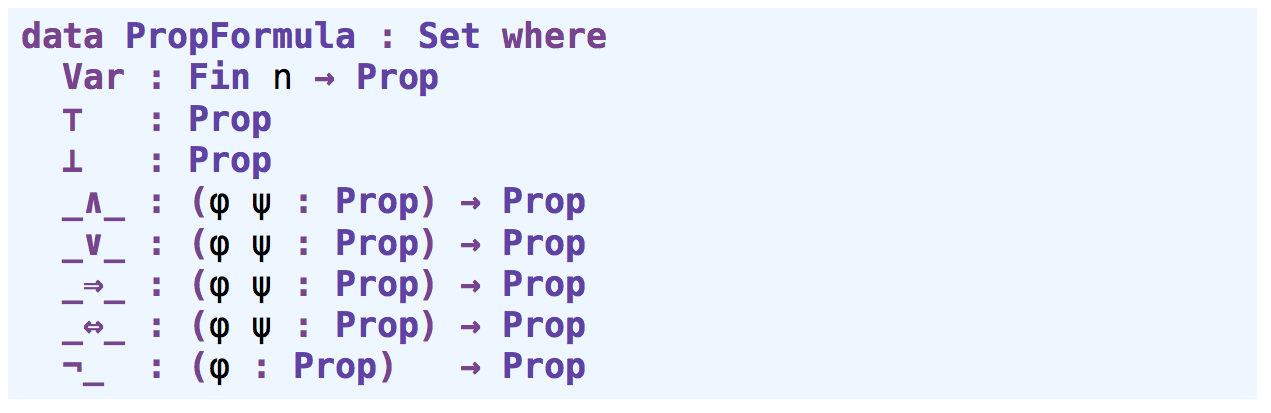
\includegraphics[width=0.95\textwidth]{prop}
\end{center}
\vfill

% {\djvu
% \begin{MyAgda}
% data Prop : Set where
%   Var : Fin n → Prop
%   ⊤   : Prop
%   ⊥   : Prop
%   _∧_ : (φ ψ : Prop) → Prop
%   _∨_ : (φ ψ : Prop) → Prop
%   _⇒_ : (φ ψ : Prop) → Prop
%   _⇔_ : (φ ψ : Prop) → Prop
%   ¬_  : (φ : Prop)   → Prop
% \end{MyAgda}
% }

\end{frame}

\begin{frame}[fragile]{Inference Rules For Propositional Logic I}

Intuitionistic Propositional Logic + PEM ($\Gamma ⊢ \varphi \vee \neg \varphi$)

\begin{columns}[t]
\column{0.33\textwidth}
  \begin{scprooftree}{0.8}
    \AxiomC{$ $}
    \RightLabel{assume}
    \UnaryInfC{$Γ , φ ⊢ φ$}
  \end{scprooftree}
\column{0.33\textwidth}
  \begin{scprooftree}{0.8}
    \AxiomC{$ $}
    \RightLabel{$⊤$-intro}
    \UnaryInfC{$Γ ⊢ ⊤$}
  \end{scprooftree}
\column{0.33\textwidth}
  \begin{scprooftree}{0.8}
\AxiomC{\,}
\RightLabel{PEM}
\UnaryInfC{$Γ ⊢ φ ∨ ¬ φ$}
\end{scprooftree}
  \end{columns}
\medskip

\begin{columns}[t]
\column{0.33\textwidth}
 \begin{scprooftree}{0.8}
    \AxiomC{$Γ ⊢ ⊥$}
    \RightLabel{$⊥$-elim}
    \UnaryInfC{$Γ ⊢ φ$}
  \end{scprooftree}
\column{0.33\textwidth}
\begin{scprooftree}{0.8}
    \AxiomC{$Γ , φ ⊢ ⊥$}
    \RightLabel{$¬$-intro}
    \UnaryInfC{$Γ ⊢ ¬ φ$}
  \end{scprooftree}
\column{0.30\textwidth}
  \begin{scprooftree}{0.8}
    \AxiomC{$Γ ⊢ ¬ φ$}
    \AxiomC{$Γ ⊢ φ$}
    \RightLabel{$¬$-elim}
    \BinaryInfC{$Γ ⊢ ⊥$}
  \end{scprooftree}
\end{columns}
\medskip
\begin{columns}[t]
\column{0.33\textwidth}
  \begin{scprooftree}{0.8}
    \AxiomC{$Γ ⊢ φ$}
    \AxiomC{$Γ ⊢ ψ$}
    \RightLabel{$\wedge$-intro}
    \BinaryInfC{$Γ ⊢ φ \wedge ψ$}
  \end{scprooftree}
  \column{0.33\textwidth}
  \begin{scprooftree}{0.8}
    \AxiomC{$Γ ⊢ φ \wedge ψ$}
    \RightLabel{$\wedge$-proj$_1$}
    \UnaryInfC{$Γ⊢ φ$}
  \end{scprooftree}
  \column{0.33\textwidth}
  \begin{scprooftree}{0.8}
    \AxiomC{$Γ ⊢ φ \wedge ψ$}
    \RightLabel{$\wedge$-proj$_2$}
    \UnaryInfC{$Γ⊢ ψ$}
  \end{scprooftree}
\end{columns}

\end{frame}

\begin{frame}[fragile]{Inference Rules For Propositional Logic II}

\begin{columns}[t]
  \column{0.40\textwidth}
  \begin{scprooftree}{1}
    \AxiomC{$Γ ⊢ φ$}
    \RightLabel{$\vee$-intro$_1$}
    \UnaryInfC{$Γ ⊢ φ \vee ψ$}
  \end{scprooftree}
  \column{0.40\textwidth}
  \begin{scprooftree}{1}
    \AxiomC{$Γ ⊢ ψ$}
    \RightLabel{$\vee$-intro$_2$}
    \UnaryInfC{$Γ ⊢ φ \vee ψ$}
  \end{scprooftree}
\end{columns}
\medskip
\begin{center}
  \begin{scprooftree}{1}
    \AxiomC{$Γ , φ ⊢ γ $}
    \AxiomC{$Γ , ψ  ⊢ γ$}
    \RightLabel{$\vee$-elim}
    \BinaryInfC{$Γ , φ \vee ψ ⊢ γ$}
  \end{scprooftree}
\end{center}
\medskip
\begin{columns}[t]
\column{0.35\textwidth}
  \begin{scprooftree}{1}
    \AxiomC{$Γ , φ ⊢ ψ$}
    \RightLabel{$\Rightarrow$-intro}
    \UnaryInfC{$Γ ⊢ φ \Rightarrow ψ$}
  \end{scprooftree}
\column{0.50\textwidth}
  \begin{scprooftree}{1}
\AxiomC{$Γ ⊢ φ \Rightarrow ψ$}
\AxiomC{$Γ ⊢ φ$}
\RightLabel{$\Rightarrow$-elim}
\BinaryInfC{$Γ ⊢ ψ$}
\end{scprooftree}
\end{columns}
\end{frame}


\begin{frame}{Other Rules}
\begin{itemize}
\item Weakening: to extend the hypotheses with additional formulas
\vskip 2mm
\begin{center}
\begin{scprooftree}{1.1}
    \AxiomC{$Γ ⊢ φ$}
    \RightLabel{weaken}
    \UnaryInfC{$Γ , ψ ⊢ φ$}
  \end{scprooftree}
\end{center}
\vskip 2mm
\item
The \abbrev{RAA} rule is the formulation of
the principle of proof by contradiction:
\vskip 2mm
\begin{center}
\begin{scprooftree}{1.1}
\AxiomC{$Γ, ¬ φ ⊢ ⊥$}
\RightLabel{RAA}
\UnaryInfC{$Γ ⊢ φ$}
\end{scprooftree}
\end{center}
\vskip 2mm
\end{itemize}
\end{frame}

\begin{frame}[fragile]{Syntactical Consequence Relation in \Agda}
\begin{itemize}
  \item Inductive family $\_⊢\_$ with two indexes: a set of propositions~$Γ$
  (the premises) and a proposition~$φ$ (the conclusion)

\begin{example}
In \cite{AgdaProp} we define $\_⊢\_$ as follows
\begin{MyAgda}
data _⊢_ : (Γ : Ctxt)(φ : Prop) → Set
  ...
  ∧-intro
    : ∀ {Γ} {φ ψ}
    → Γ ⊢ φ → Γ ⊢ ψ
    → Γ ⊢ φ ∧ ψ

  ∧-proj₁
    : ∀ {Γ} {φ ψ}
    → Γ ⊢ φ ∧ ψ
    → Γ ⊢ φ

  ∧-proj₂
    : ∀ {Γ} {φ ψ}
    → Γ ⊢ φ ∧ ψ
    → Γ ⊢ ψ
  ...
\end{MyAgda}
\end{example}
\end{itemize}
\end{frame}

\begin{frame}[fragile]{Reconstructing \Metis Rules in Type Theory}

Let \textrm{metisRule} be a \Metis inference rule. We define the function \fun{metisRule} in type theory which has the following pattern\footnote{
\Source and \Target as synonyms of the \Prop type to describe in the
function types the role of the arguments}:
\begin{equation*}
  \begin{aligned}
  &\hspace{.495mm}\fun{metisRule} : \Source → \Target → \Prop\\
  &\begin{array}{ll}
  \fun{metisRule}~φ~ψ\ &=
      \begin{cases}
      ψ, &\text{if }\fun{metisRule} \text{ built }ψ\text{ by applying inference}\\
         &\text{rules to }φ;\\
      φ, &\text{otherwise;}
      \end{cases}
  \end{array}
  \end{aligned}
\end{equation*}

To justify all transformations done by the \fun{metisRule} rule, we prove
its soundness with a theorem like the following:
\begin{equation*}
  \text{If }Γ ⊢ φ \text{ then }Γ ⊢ \fun{metisRule}~φ~ψ, \text{ where } ψ : \Target.
\end{equation*}
\end{frame}

% --------------------------------------------------------------------
\begin{frame}[fragile]{Reconstructing a \Metis Inference Rule}

The \clausify rule transforms a formula into its clausal normal form.

\begin{example}

In the following \TSTP derivation by \Metis, we see how
\clausify transforms the \texttt{norm₀} formula to get \texttt{norm₁} formula.

\begin{verbatim}
fof(norm₀, ¬ p ∨ (q ∧ r) ...
fof(norm₁, (¬ p ∨ q) ∧ (¬ p ∨ r), inf(clausify, norm₀)).
\end{verbatim}

\end{example}

\begin{mainth}
   Let $ψ : \Target$. If $Γ ⊢ φ$ then $Γ ⊢ \fclausify~φ~ψ$, where
  \begin{equation*}
  \begin{aligned}
  &\hspace{.495mm}\fclausify : \Source → \Target → \Prop\\
  &\begin{array}{llll}
  \fclausify~φ~ψ &=
         \begin{cases}
        ψ, &\text{ if }φ≡ψ;\\
        \freorder_{∧∨}~(\fcnf~φ)~ψ, &\text{ otherwise.}
      \end{cases}
  \end{array}
  \end{aligned}
  \end{equation*}
\end{mainth}

% \begin{proof}
% If $φ ≡ ψ$, $Γ ⊢ \fclausify~φ~ψ$ normalizes to $Γ ⊢ ψ$. The conclusion follows by applying the $\fsubst$ lemma. Otherwise, we use Lemma~\ref{lem:reorder-and-or} and Lemma~\ref{lem:cnf}.
% \end{proof}

\end{frame}

% --------------------------------------------------------------------
\begin{frame}[fragile]{Sketch of the \Metis Algorithm}
\begin{center}
\scalebox{0.75}{
\begin{minipage}{\textwidth}
\begin{algorithm}[H]
\caption{\Metis refutation strategy}
\begin{algorithmic}[Metis]
\Procedure{metis}{}\newline
  \textbf{input:} the \textrm{goal} and a set of \emph{premises} $a_1,\cdots, a_n$
  \newline
  \textbf{output:} maybe a derivation when $a_1,\cdots,a_n \vdash \textrm{goal}$, otherwise nothing. \newline
    \State{strip the goal into a list of \emph{subgoals} $s_i$}
    \For{each subgoal $s_i$}
    \State{try to find by a refutation for $\neg s_i$:}
    \State{\ \ \ apply clausification for the negated subgoal $¬ s_i$}
    \ \ \ \If{a premise $a_j$ is relevant}
    \ \ \ \ \ \State{apply clausification to $a_j$}
    \ \ \ \EndIf
    \State{\ \ \ application of \Metis inference rules}
    \ \ \  \If{a contradiction can be derived from the assumptions}
    \ \ \ \ \ \State{keep the refutation and continue with the others subgoals}
   \ \ \ \ \ \Else
    \ \ \ \ \ \State{exit without a proof.}
    \EndIf
    \EndFor
    \State{print the conjecture and the premises}
    \State{print each refutation for each negated subgoal}
    \EndProcedure
\end{algorithmic}
\end{algorithm}
\end{minipage}
}
\end{center}
\end{frame}


\begin{frame}{Some Challenges}
\begin{itemize}
  \item Formalization
\begin{itemize}
  \item Understanding the \Metis reasoning without a proper
  documentation or description from the \Metis author
  \item Terminating of functions that reconstruct \Metis inference rules
  \item Intuitionistic logic implementation
\end{itemize}
\item Software related
\begin{itemize}
  \item Parsing of \TSTP derivations
  \item Printing valid \Agda files
\end{itemize}

\end{itemize}
\end{frame}

\begin{frame}[fragile]{Complete Example}
The problem\footnote{Problem No.~13 in Disjunction Section in \cite{Prieto-Cubides2017}}:
\begin{equation*}
(p \Rightarrow q) \wedge (q \Rightarrow p) ⊢ (p \vee q) \Rightarrow (p \wedge q)
\end{equation*}
In \TPTP syntax:
\begin{verbatim}
  fof(a₁, axiom, (p ⇒ q) ∧ (q ⇒ p)).
  fof(goal, conjecture, (p ∨ q) ⇒ (p ∧ q)).
\end{verbatim}
Its \TSTP solution using \Metis:
\begin{verbatim}
  fof(a₁, axiom, (p ⇒ q) ∧ (q ⇒ p)).
  fof(goal, conjecture, (p ∨ q) ⇒ (p ∧ q))).
  fof(s₁, (p ∨ q) ⇒ p, inf(strip, goal)).
  fof(s₂, ((p ∨ q) ∧ p) ⇒ q, inf(strip, goal)).
  ...
\end{verbatim}
\end{frame}

\begin{frame}[fragile,plain]
\begin{verbatim}
  fof(premise, axiom, (p ⊃ q) ∧ (q ⊃ p)).
  fof(goal, conjecture, (p ∨ q) ⊃ (p ∧ q)).
  fof(s₀, (p ∨ q) ⊃ p, inf(strip, goal)).
  fof(s₁, ((p ∨ q) ∧ p) ⊃ q, inf(strip, goal)).
  fof(neg₀, ¬ ((p ∨ q) ⊃ p), inf(negate, s₀)).
  fof(n₀₀, (¬ p ∨ q) ∧ (¬ q ∨ p), inf(canonicalize, premise)).
  fof(n₀₁, ¬ q ∨ p, inf(conjunct, n₀₀)).
  fof(n₀₂, ¬ p ∧ (p ∨ q), inf(canonicalize, neg₀)).
  fof(n₀₃, p ∨ q, inf(conjunct, n₀₂)).
  fof(n₀₄, ¬ p, inf(conjunct, n₀₂)).
  fof(n₀₅, q, inf(simplify, [n₀₃, n₀₄])).
  cnf(r₀₀, ¬ q ∨ p, inf(canonicalize, n₀₁)).
  cnf(r₀₁, q, inf(canonicalize, n₀₅)).
  cnf(r₀₂, p, inf(resolve, q, [r₀₁, r₀₀])).
  cnf(r₀₃, ¬ p, inf(canonicalize, n₀₄)).
  cnf(r₀₄, ⊥, inf(resolve, p, [r₀₂, r₀₃])).
  fof(neg₁, ¬ ((p ∨ q) ∧ p) ⊃ q), inf(negate, s₁)).
  fof(n₁₀, ¬ q ∧ p ∧ (p ∨ q), inf(canonicalize, neg₁)).
  fof(n₁₁, (¬ p ∨ q) ∧ (¬ q ∨ p), inf(canonicalize, premise)).
  fof(n₁₂, ¬ p ∨ q, inf(conjunct, n₁₁)).
  fof(n₁₃, ⊥, inf(simplify, [n₁₀, n₁₂])).
  cnf(r₁₀, ⊥, inf(canonicalize, n₁₃)).
\end{verbatim}
\end{frame}

\begin{frame}[fragile]{\TSTP Refutation of Subgoal No. 1}
\begin{verbatim}
  fof(premise, axiom, (p ⊃ q) ∧ (q ⊃ p)).
  fof(goal, conjecture, (p ∨ q) ⊃ (p ∧ q)).
  fof(s₀, (p ∨ q) ⊃ p, inf(strip, goal)).
  ...
  fof(neg₀, ¬ ((p ∨ q) ⊃ p), inf(negate, s₀)).
  fof(n₀₀, (¬ p ∨ q) ∧ (¬ q ∨ p), inf(canonicalize, premise)).
  fof(n₀₁, ¬ q ∨ p, inf(conjunct, n₀₀)).
  fof(n₀₂, ¬ p ∧ (p ∨ q), inf(canonicalize, neg₀)).
  fof(n₀₃, p ∨ q, inf(conjunct, n₀₂)).
  fof(n₀₄, ¬ p, inf(conjunct, n₀₂)).
  fof(n₀₅, q, inf(simplify, [n₀₃, n₀₄])).
  cnf(r₀₀, ¬ q ∨ p, inf(canonicalize, n₀₁)).
  cnf(r₀₁, q, inf(canonicalize, n₀₅)).
  cnf(r₀₂, p, inf(resolve, q, [r₀₁, r₀₀])).
  cnf(r₀₃, ¬ p, inf(canonicalize, n₀₄)).
  cnf(r₀₄, ⊥, inf(resolve, p, [r₀₂, r₀₃])).
\end{verbatim}
\end{frame}

\begin{frame}[fragile]{Refutation Tree for $s₀$}

\begin{verbatim}
  fof(premise, axiom, (p ⊃ q) ∧ (q ⊃ p)).
  ...
  fof(n₀₀, (¬ p ∨ q) ∧ (¬ q ∨ p), inf(canonicalize, premise)).
  fof(n₀₁, ¬ q ∨ p, inf(conjunct, n₀₀)).
  ...
\end{verbatim}

\begin{prooftree}
\AxiomC{}
\RightLabel{axiom premise}
\UnaryInfC{$\Gamma \vdash (p \Rightarrow q) \wedge (q \Rightarrow p)$}
\RightLabel{weaken}
\UnaryInfC{$\Gamma, \neg s_1 \vdash (p \Rightarrow q) \wedge (q \Rightarrow p)$}
\LeftLabel{$(\mathcal{D}_1)$\hspace{1.5cm}}
\RightLabel{canonicalize}
\UnaryInfC{$\Gamma, \neg s_1 \vdash (\neg p \vee q) \wedge (\neg q \vee p)$}
\RightLabel{conjunct}
\UnaryInfC{$\Gamma, \neg s_1 \vdash \neg q \vee p$}
\end{prooftree}

\end{frame}

\begin{frame}[fragile]
\begin{verbatim}
...
fof(s₁, (p ∨ q) ⇒ p, inf(strip, goal)).
fof(neg₁, ¬ ((p ∨ q) ⇒ p), inf(negate, s₁)).
...
fof(n02, ¬ p ∧ (p ∨ q), inf(canonicalize, neg₁)).
fof(n03, p ∨ q, inf(conjunct, n02)).
fof(n04, ¬ p, inf(conjunct, n02)).
...
\end{verbatim}
\begin{prooftree}
\AxiomC{}
\RightLabel{assume}
\UnaryInfC{$\Gamma, \neg s_1 \vdash \neg s_1$}
\LeftLabel{$(\mathcal{D}_2)$\hspace{1.5cm}}
\RightLabel{canonicalize}
\UnaryInfC{$\Gamma, \neg s_1 \vdash \neg p \wedge (p \vee q)$}
\RightLabel{conjunct}
\UnaryInfC{$\Gamma, \neg s_1 \vdash p \vee q$}
\end{prooftree}

% ($\mathcal{D}_3$)
\begin{prooftree}
\AxiomC{}
\RightLabel{assume $\neg s_1$}
\UnaryInfC{$\Gamma, \neg s_1 \vdash \neg s_1$}
% \UnaryInfC{$\Gamma, \neg s_1 \vdash (p \vee q) \Rightarrow p$}
\LeftLabel{$(\mathcal{D}_3)$\hspace{1.5cm}}
\RightLabel{canonicalize}
\UnaryInfC{$\Gamma, \neg s_1 \vdash \neg p \wedge (p \vee q)$}
\RightLabel{conjunct}
\UnaryInfC{$\Gamma, \neg s_1 \vdash \neg p$}
\end{prooftree}
\end{frame}

\begin{frame}
\vfill
\begin{prooftree}
\AxiomC{$\mathcal{D}_2$}
\UnaryInfC{$\Gamma, \neg s_1 \vdash p \vee q$}
%
\AxiomC{$\mathcal{D}_3$}
\UnaryInfC{$\Gamma, \neg s_1 \vdash \neg p$}
%
\LeftLabel{$(\mathcal{D}_4)$\hspace{1.5cm}}
\RightLabel{simplify}
\BinaryInfC{$\Gamma, \neg s_1 \vdash q$}
\end{prooftree}
\vfill
\begin{prooftree}
\AxiomC{$\mathcal{D}_1$}
\UnaryInfC{$\Gamma, \neg s_1 \vdash \neg q \vee p$}
\AxiomC{$\mathcal{D}_4$}
\UnaryInfC{$\Gamma, \neg s_1 \vdash q$}
\RightLabel{resolve $q$}
\BinaryInfC{$\Gamma, \neg s_1 \vdash p$}
\RightLabel{}
\AxiomC{$\mathcal{D}_3$}
\UnaryInfC{$\Gamma, \neg s_1 \vdash \neg p$}
\RightLabel{resolve $p$}
\LeftLabel{$(\mathcal{R}_1)$\hspace{1.5cm}}
\BinaryInfC{$\Gamma, \neg s_1 \vdash \bot$}
\RightLabel{RAA}
\UnaryInfC{$\Gamma \vdash s_1$}
\end{prooftree}
\vfill
\end{frame}

\begin{frame}[fragile]
  {Tree for the Subgoal No.~2: $((p ∨ q) ∧ p) ⇒ q$}
\begin{verbatim}
fof(s₂, ((p ∨ q) ∧ p) ⇒ q, inf(strip, goal)).
fof(neg₂, ¬ (((p ∨ q) ∧ p) ⇒ q), inf(negate, s2)).
fof(n10, ¬ q ∧ p ∧ (p ∨ q), inf(canonicalize, neg₂)).
fof(n11, (¬ p ∨ q) ∧ (¬ q ∨ p), inf(canonicalize, a₁)).
fof(n12, ¬ p ∨ q, inf(conjunct, n11)).
fof(n13, ⊥, inf(simplify,[n10, n12])).
cnf(r10, ⊥, inf(canonicalize, n13)).
\end{verbatim}

\begin{scprooftree}{0.7}
\AxiomC{}
\RightLabel{assume ($\neg s_2)$}
\UnaryInfC{$\Gamma ,\neg s_2 \vdash \neg s_2$}
\RightLabel{canonicalize}
\UnaryInfC{$\Gamma, \neg s_2\vdash \neg q \wedge p \wedge (p \vee q)$}
\AxiomC{}
\RightLabel{axiom $a_1$}
\UnaryInfC{$\Gamma \vdash (p \Rightarrow q) \wedge (q \Rightarrow p)$}
\RightLabel{weaken}
\UnaryInfC{$\Gamma, \neg s_2 \vdash (p\Rightarrow q) \wedge (q \Rightarrow p)$}
\RightLabel{canonicalize}
\UnaryInfC{$\Gamma, \neg s_2 \vdash (\neg p \vee q) \wedge (\neg q \vee p)$}
\RightLabel{conjunct}
\UnaryInfC{$\Gamma, \neg s_2 \vdash \neg p \vee q$}
\LeftLabel{$(\mathcal{R_2})$\hspace{1cm}}
\RightLabel{simplify}
\BinaryInfC{$\Gamma, \neg s_2 \vdash \bot$}
\RightLabel{RAA}
\UnaryInfC{$\Gamma \vdash s_2$}
\end{scprooftree}

\end{frame}

\begin{frame}[fragile]{Summarizing the Example}
The problem was:
\begin{equation*}
(p \Rightarrow q) \wedge (q \Rightarrow p) ⊢ (p \vee q) \Rightarrow (p \wedge q)
\end{equation*}
Its \TSTP solution using \Metis was:
\begin{verbatim}
  fof(a₁, axiom, (p ⇒ q) ∧ (q ⇒ p)).
  fof(goal, conjecture, (p ∨ q) ⇒ (p ∧ q))).
  fof(s₁, (p ∨ q) ⇒ p, inf(strip, goal)).
  fof(s₂, ((p ∨ q) ∧ p) ⇒ q, inf(strip, goal)).
  ...
\end{verbatim}
The proof is:
\begin{prooftree}
\AxiomC{}
\RightLabel{strip}
\UnaryInfC{$\Gamma \vdash (s_1 \wedge s_2) \Rightarrow \text{goal}$}
\AxiomC{$\mathcal{R_1}$}
\UnaryInfC{$\Gamma \vdash s_1$}
\AxiomC{$\mathcal{R_2}$}
\UnaryInfC{$\Gamma \vdash s_2$}
\RightLabel{$\wedge$-intro}
\BinaryInfC{$\Gamma \vdash s_1 \wedge s_2$}
\RightLabel{$\Rightarrow$-elim}
\BinaryInfC{$\Gamma \vdash \text{goal}$}
\end{prooftree}
\vfill
(Live example using Agda and Athena)
\end{frame}


\begin{frame}[label=future-work]{Future Work}
Further research directions include, but are not limited to:

\begin{itemize}
\item improve the performance of the \canonicalize rule
\item extend the proof-reconstruction presented in this paper to
  \begin{itemize}
    \item support the identity theory
    \item support other \ATPs for propositional logic like \name{EProver}
     or \name{Z3}.\\
     See Kanso's Ph.D. thesis~\cite{Kanso2012}
    \item support \Metis first-order proofs
  \end{itemize}
\end{itemize}
\end{frame}

\begin{frame}{Related Work}
In type theory:
\begin{itemize}
  \item \citeauthor{Kanso2012} in \cite{Kanso2012} reconstructs in \Agda propositional proofs generated by \name{EProver} and \name{Z3}
  \item \citeauthor{foster2011integrating} in \cite{foster2011integrating}
  describe proof-reconstruction in \Agda for equational logic of \name{Waldmeister} prover
  \item \citeauthor{Bezem2002} in \cite{Bezem2002} transform a proof produced by the first-order prover \name{Bliksem} in a \name{Coq} proof-term
\end{itemize}
In classical logic:
\begin{itemize}
\item \citeauthor{paulson2007source} in \cite{paulson2007source} introduce
\name{SledgeHammer}, a tool ables to reconstructs proofs of well-known \ATPs: \name{EProver}, \name{Vampire}, among others using \name{SystemOnTPTP} server
\item \citeauthor{Hurd1999} in \cite{Hurd1999} integrates the first-order resolution prover \name{Gandalf} prover for \name{HOL} proof-assistant
\item \citeauthor{kaliszyk2013} in \cite{kaliszyk2013} reconstruct proofs
of different \ATPs for \name{HOL Light}
\end{itemize}
\end{frame}

\begin{frame}[allowframebreaks]{References}
\printbibliography
\end{frame}

\begin{frame}{BONUS SLIDES}
\end{frame}

\begin{frame}[fragile, label=tptp-syntax]{\TPTP Syntax}
  {Thousands of Problems for Theorem Provers}

  \begin{itemize}
  \item Is a language\footnote{\url{http://www.cs.miami.edu/~tptp/TPTP/SyntaxBNF.html}.}  to encode problems
  \item Is the input of the \ATPs
  \item Annotated formulas with the form
   \begin{center}
\begin{verbatim}
language(name, role, formula).
\end{verbatim}
    \end{center}
    \begin{itemize}
      \item[\texttt{language}] FOF or CNF
      \item[\texttt{name}] to identify the formula within the problem
      \item[\texttt{role}] axiom, definition, hypothesis, conjecture
      \item[\texttt{formula}] formula in \TPTP format
    \end{itemize}
  \end{itemize}
\end{frame}

\begin{frame}[label=metis, fragile]{\Metis Theorem Prover}
\Metis is an automatic theorem prover for first-order logic with
equality.
\begin{block}{}
  \begin{itemize}
    \item \href{https://github.com/gilith/metis}{Open source} implemented
    % in \texttt{Standard ML}
    \item Reads problems in \TPTP format
    \item Outputs \textit{detailed} proofs in \TSTP format
    \item For the propositional logic, \Metis has only three inference rules:
      \vfill
      \begin{prooftree}
        \AxiomC{}
        \RightLabel{axiom $φ₁, \cdots,φₙ$}
        \UnaryInfC{$\Gamma ⊢ φ₁ ∨ \cdots ∨ φₙ$}
      \end{prooftree}
      \vfill
      \begin{prooftree}
        \AxiomC{}
        \RightLabel{assume $\varphi$}
        \UnaryInfC{$\Gamma ⊢ \varphi \vee \neg \varphi$}
      \end{prooftree}
      \vfill
      \begin{scprooftree}{0.8}
        \AxiomC{$\Gamma ⊢ φ₁ ∨ \cdots ∨ l ∨ \cdots  ∨ φₙ$}
        \AxiomC{$\Gamma ⊢ ψ₁ ∨ \cdots ∨ ¬ l ∨ \cdots ∨ ψₘ$}
        \RightLabel{resolve $l$}
        \BinaryInfC{$\Gamma ⊢ φ₁ ∨ \cdots ∨ φₙ ∨ ψ₁ ∨ \cdots ∨ ψₘ$}
      \end{scprooftree}
  \vfill
  \end{itemize}
\vfill
\end{block}

\end{frame}

\begin{frame}[fragile]{\TSTP Syntax}
A \TSTP derivation\footnote{\url{http://www.cs.miami.edu/~tptp/TPTP/QuickGuide/Derivations.html}.}
\begin{itemize}
  \item Is a \textbf{D}irected \textbf{A}cyclic \textbf{G}raph where
  \begin{itemize}
    \item[\texttt{leaf}] is a formula from the \TPTP input
    \item[\texttt{node}] is a formula inferred from parent formula
    \item[\texttt{root}] the final derived formula
  \end{itemize}
  \item Is a list of annotated formulas with the form
  \end{itemize}

\begin{verbatim}
  language(name, role, formula, source [,useful info]).
\end{verbatim}

where \texttt{\color{blu} source} typically is an inference record
\begin{verbatim}
  inference(rule, useful info, parents).
\end{verbatim}
\end{frame}


\begin{frame}[fragile, label=tstp-example]{Another \TSTP Example}

\begin{itemize}
  \item Proof found by \Metis for the problem $p ⊢ p$
{\small
\begin{verbatim}
$ metis --show proof problem.tptp
fof(a, axiom, p).
fof(goal, conjecture, p).
fof(subgoal_0, plain, p),
  inference(strip, [], [goal])).
fof(negate_0_0, plain, ~ p,
  inference(negate, [], [subgoal_0])).
fof(normalize_0_0, plain, ~ p,
  inference(canonicalize, [], [negate_0_0])).
fof(normalize_0_1, plain, p,
  inference(canonicalize, [], [a])).
fof(normalize_0_2, plain, $false,
  inference(simplify, [],
    [normalize_0_0, normalize_0_1])).
cnf(refute_0_0, plain, $false,
    inference(canonicalize, [], [normalize_0_2])).
\end{verbatim}
}
\end{itemize}
\end{frame}


\begin{frame}[fragile, label=tstp-dag]{DAG Example}
\vfill
By refutation, we proved $p ⊢ p$:

\begin{columns}
\begin{column}{0.5\textwidth}

\begin{prooftree}
\AxiomC{}
\RightLabel{assume}
\UnaryInfC{$¬ p$}
\RightLabel{strip}
\UnaryInfC{$¬ p$}
\AxiomC{}
\RightLabel{axiom}
\UnaryInfC{$p$}
\RightLabel{canonicalize}
\UnaryInfC{$p$}
\RightLabel{simplify}
\BinaryInfC{$⊥$}
\RightLabel{canonicalize}
\UnaryInfC{$⊥$}
\end{prooftree}
\end{column}
\begin{column}{0.5\textwidth}  %%<--- here
    \begin{center}
    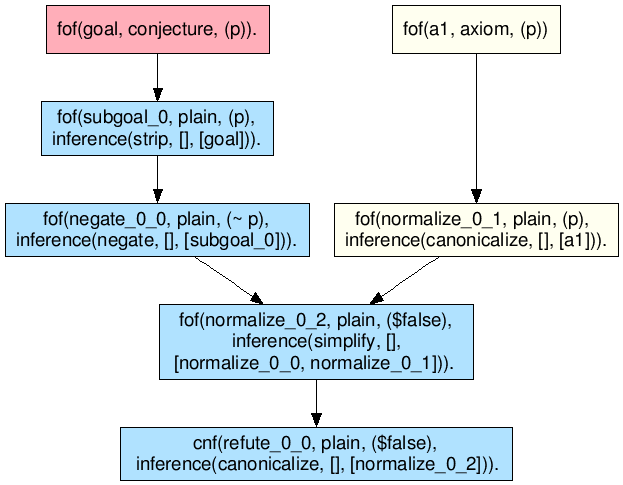
\includegraphics[height=0.8\textwidth]{figures/derivation.png}
     \end{center}
\end{column}
\end{columns}
\vfill
\end{frame}


\begin{frame}[fragile]{\Athena tool}

Is an \Haskell program that translates proofs given by \Metis in \TSTP
format to \Agda code\\

\begin{itemize}
    \item Parsing of \TSTP language
    \item Creation and analysis of \hyperlink{tstp-dag}{\textbf{DAG}} derivations
    \item Analysis of inference rules used in the \TSTP derivation
    \item \Agda code generation
\begin{table}[!ht]

\begin{center}
\scalebox{0.8}{
{\renewcommand{\arraystretch}{1.3}%
\begin{tabular}{|ll| }
\hline
\textbf{Library} & \textbf{Purpose} \\
\hline
\texttt{agda-prop}& axioms and theorems of classical propositional logic\\
\texttt{agda-metis} & versions of the inference rules used by \Metis\\
\hline
\end{tabular}}
}
\end{center}
\label{tab:library}
\end{table}

\end{itemize}
\end{frame}




\begin{frame}[fragile, label=conjunct-thm]{\texttt{agda-metis}: Conjunct Inference
  \footnote{\url{https://github.com/jonaprieto/agda-metis}.}
  }

\vfill
\begin{itemize}
\item Definition
\begin{equation*}
\text{\color{blu!40!black}conjunct}(\overbrace{\varphi_1 ∧ ⋯ ∧ \varphi_n}^{\varphi}, \psi)
= \begin{cases}
\varphi_{i} \ \ \ \ \text{if }\psi\text{ is equal to some }\varphi_i\\
\varphi    \ \ \ \ \text{otherwise}
\end{cases}
\end{equation*}

\pause
\item Inference rules involved
\begin{center}
\begin{columns}
\begin{column}{0.42\textwidth}

 \begin{prooftree}
  \AxiomC{$\varphi_1 ∧ \varphi_2$}
  \RightLabel{\scriptsize $∧$-\texttt{proj}$₁$}
  \UnaryInfC{$\varphi_1$}
  \end{prooftree}
\end{column}

\begin{column}{0.42\textwidth}
 \begin{prooftree}
  \AxiomC{$\varphi_1 ∧ \varphi_2$}
  \RightLabel{\scriptsize $∧$-\texttt{proj}$₂$}
  \UnaryInfC{$\varphi₂$}
  \end{prooftree}
\end{column}

\begin{column}{0.2\textwidth}  %%<--- here
  \begin{tikzpicture}[
    ->
  , >=stealth'
  , shorten >=1pt
  , auto
%  , node distance=2.8cm
  , thick
  , overlay
  , remember picture
    , transform canvas={scale=.75}
    ]
  \tikzset{shift={(current page.center)}, xshift=4.5cm,yshift=0cm}

  \node[fill=blu!45!black,draw=none,text=white]  (phi)                     {$\varphi$};
  \node[fill=blu!45!black,draw=none,text=white]  (phi1) [below left =1.3cm and 0.1cm of phi]  {$\varphi_1$};
  \node[fill=blu!45!black,draw=none,text=white]  (phi2) [below right=1.3cm and 0.1cm of phi]  {$\varphi_2$};
  \node[fill=blu!45!black,draw=none,text=white]  (phi3)  [below left =1.3cm and 0.1cm of phi2]  {$\varphi_3$};
  \node[fill=blu!45!black,draw=none,text=white]  (phi4)  [below right =1.3cm and 0.1cm of phi2]  {$\varphi_4$};

  \path[every node/.style={sloped,anchor=south,auto=false}]
        (phi) edge node {\tiny $∧$-\texttt{proj}$₁$} (phi1)
        (phi) edge node {\tiny $∧$-\texttt{proj}$₂$} (phi2)
        (phi2) edge node {\tiny $∧$-\texttt{proj}$₁$} (phi3)
        (phi2) edge node {\tiny $∧$-\texttt{proj}$₂$} (phi4);

\end{tikzpicture}
\end{column}
\end{columns}
\end{center}
\vskip 2mm

\item Example
\[ \varphi := \varphi_1 ∧ \overbrace{(\varphi_3 ∧ \varphi_4)}^{\varphi_2}\]

\begin{itemize}

\item
\fun{conjunct}$(\varphi , \varphi_3 ∧ \varphi_1) ≡ \varphi$
\vskip 3mm
\item
\fun{conjunct}$(\varphi , \varphi_3)      ≡ \varphi_3$
\vskip 3mm
\item
\fun{conjunct}$(\varphi , \varphi_2)      ≡ \varphi_2$
\vskip 3mm
\end{itemize}

\end{itemize}
\end{frame}





% \begin{frame}[fragile, label=hammer]{Related Work}
% \begin{block}{SledgeHammer} \citep{Paulson2007}
% \begin{itemize}
% \item \texttt{Isabelle}/\texttt{HOL} mature tool
% \item \Metis ported within \texttt{Isabelle/HOL}
% \item Reconstruct proofs of well-known ATPs: \texttt{EProver}, \texttt{Vampire},
% among others using \texttt{SystemOnTPTP} server
% \end{itemize}
% \end{block}

% \begin{block}{Integrating \texttt{Waldmeister} into \Agda} \citep{Foster2011}
% \begin{itemize}
%   \item Framework for a integration between \Agda and ATPs
%   \begin{itemize}
%     \item Equational Logic
%     \item Reflection Layers
%   \end{itemize}
%   \item Source code is not available\footnote{\url{http://simon-foster.staff.shef.ac.uk/agdaatp}.}
%   \end{itemize}
% \end{block}
% \end{frame}



% \begin{frame}[fragile]{Related Work: \texttt{Apia}}
%   {Proving First-Order theorems written in \Agda using automatic
%   theorem provers for First-Order Logic}

% \only<1>{At the moment, the communication between \Agda and
% the ATPs is unidirectional because the ATPs are being used as oracles \citep{Sicard2015}
% \vfill
% }
% \only<1>{
% \inputminted{cagda}{Or.agda}
% \begin{tikzpicture}[overlay, remember picture, scale=0.5]
% \tikzset{shift={(current page.center)}, xshift=6cm,yshift=-2cm}
% \node(agdafile) at (0,0){
%   
\includegraphics[scale=0.8]{figures/agda-pragmas}};
% \end{tikzpicture}
% }

% \begin{tikzpicture}

% \only<2->{ \node(agdafile) at (0,0){
%   
\includegraphics[scale=0.8]{figures/agda-pragmas}}};

% \only<2->{
%   \node[right=1cm of agdafile] (eagda){
%   
\includegraphics[scale=0.8]{figures/eagda}
%   \footnote{\url{https://github.com/asr/eagda}.}
%   }
% };

% \only<2->{
% \node[right=1cm of eagda] (agdai){
%   
\includegraphics[scale=0.8]{figures/agdai}
%   }
% };

% \only<3->{
%   \node[below=0.4cm of agdai] (apia){
%   
\includegraphics[scale=0.8]{figures/apia}
%   \footnote{\url{https://github.com/asr/apia}.}}
%   };

% \only<4->{
%   \node[below= 0.4cm of eagda] (tptp)
%     {
\includegraphics[scale=0.8]{figures/tptp}}};

% \only<5->{ \node[below = 0.8cm of apia] (atp)
%   {
\includegraphics[scale=0.8]{figures/atp}
%   \footnote{\url{http://github.com/jonaprieto/online-atps}.}}
%   };

% \only<7->{ \node[left= 2cm of atp, rectangle, text=white,fill=black, align=left, font=\small] (proved)
% {
% \texttt{\$ agda Or.agda}\\
% \texttt{\$ apia Or.agda --atp=online-metis}\\
% \texttt{Metis---2.3 proved the conjecture}
%   }
% };

% \only<2->{\draw[->, ultra thick] (agdafile) to (eagda)};
% \only<2->{\draw[->, ultra thick] (eagda) to (agdai)};
% \only<3->{\draw[->, ultra thick] (agdai) to (apia)};
% \only<4->{\draw[->, very thick, dashed, gray] (apia) to (tptp)};
% \only<5->{\draw[->, very thick, dashed, gray] (tptp) to (atp)};
% \only<6->{\draw[->, very thick, dashed, gray] (atp) to (apia)};
% \end{tikzpicture}
% \end{frame}


% \begin{frame}[fragile,label=metis-inference-rules]{\Metis Inference Rules}
% \vfill
% \begin{prooftree}
% \AxiomC{}
% \RightLabel{axiom}
% \UnaryInfC{$C$}
% \end{prooftree}
% \vfill
% \begin{prooftree}
% \AxiomC{}
% \RightLabel{assume $L$}
% \UnaryInfC{$L \vee \neg L$}
% \end{prooftree}
% \vfill
% \begin{prooftree}
% \AxiomC{$C$}
% \RightLabel{subst $σ$}
% \UnaryInfC{$σC$}
% \end{prooftree}
% \vfill
% \begin{prooftree}
% \AxiomC{$L \vee C$}
% \AxiomC{$\neg L \vee D$}
% \RightLabel{resolve $L$}
% \BinaryInfC{$C \vee D$}
% \end{prooftree}
% \vfill
% \begin{prooftree}
% \AxiomC{}
% \RightLabel{refl $t$}
% \UnaryInfC{$t = t$}
% \end{prooftree}
% \vfill
% \begin{prooftree}
% \AxiomC{}
% \RightLabel{eq $L$ $p$ $t$}
% \UnaryInfC{$\Gamma, \neg (L[p] = t) \vee \neg L \vee L[ p ↦ t]$}
% \end{prooftree}
% \vfill
%  \begin{tikzpicture}[overlay, remember picture, scale=0.5]
%     \tikzset{shift={(current page.center)}, xshift=11.8cm,yshift=-8.4cm}
%     \node[fill=blu,text=white, hyperlink node = metis]
%       (go) at (0,0) {\tiny Go Back};
%   \end{tikzpicture}
% \end{frame}
\end{document}
